%=================================================
\chapter{Refactoring Documentation (Point 7)}
%=================================================

This chapter documents individual refactorings contributed by each team
member. Each refactoring includes the context, before/after code,
rationale, and impact on quality attributes.

Each team member has performed and documented at least \textbf{three major
refactorings} as required by the project rubric. The refactorings are
categorized by type and include measurable quality impacts.

\begin{figure}[h]
  \centering
  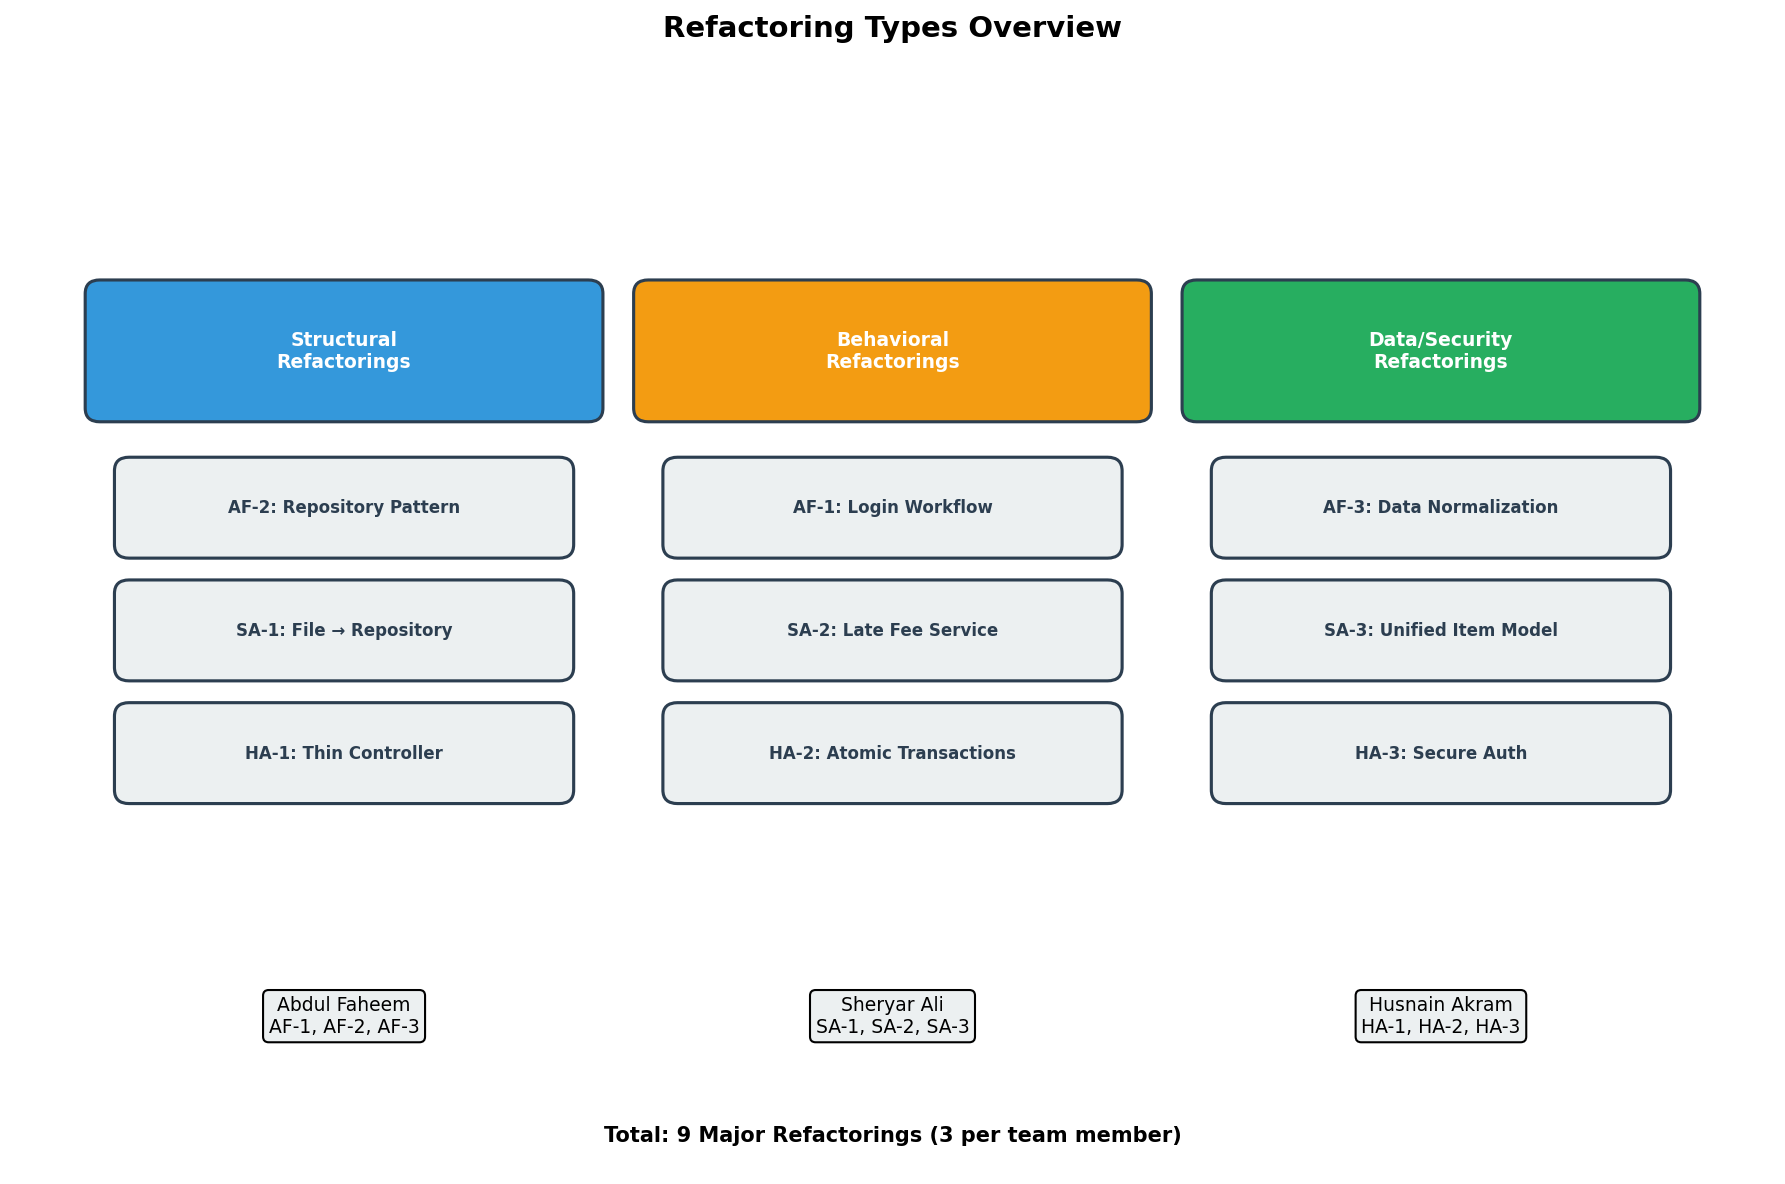
\includegraphics[width=0.95\textwidth]{images/refactoring_overview.png}
  \caption{Overview of Refactoring Types -- Distribution of refactorings across
           structural, behavioral, and data categories by team member.}
  \label{fig:refactoring-overview}
\end{figure}

\section{Refactoring Summary}

\begin{table}[h]
  \centering
  \caption{Summary of Individual Refactorings}
  \begin{tabular}{p{3.5cm} p{1.5cm} p{4cm} p{4cm}}
    \toprule
    \textbf{Member} & \textbf{ID} & \textbf{Refactoring} & \textbf{Type} \\
    \midrule
    Abdul Faheem & AF--1 & Login Workflow Clarification & Behavioral \\
    (22i--2629)  & AF--2 & Repository Abstraction & Structural \\
                 & AF--3 & Data Normalization (1NF) & Data \\
    \midrule
    Sheryar Ali  & SA--1 & File Write to Repository & Structural \\
    (22i--2623)  & SA--2 & Late-Fee Service Extraction & Behavioral \\
                 & SA--3 & Unified Item Model & Data \\
    \midrule
    Husnain Akram & HA--1 & Thin Controller Pattern & Structural \\
    (22i--2464)   & HA--2 & Atomic Transaction Service & Behavioral \\
                  & HA--3 & Secure Authentication & Security \\
    \bottomrule
  \end{tabular}
\end{table}

%=========================================================
\section{Abdul Faheem (22i--2629)}
%=========================================================

\subsection{AF--1: Clarify Login Workflow with Explicit Role Check}

\textbf{Context:}
The legacy \texttt{Login\_Interface.java} directly called
\texttt{POSSystem.logIn(...)} and relied on implicit global state to
determine which UI to show next (Cashier vs Admin).

\textbf{Before (Legacy Java):}
\begin{lstlisting}[language=Java]
// Login_Interface.java
if (POSSystem.logIn(username, password)) {
    // role determined by global POSSystem.role
    if (POSSystem.role.equals("Admin")) {
        new Admin_Interface();
    } else {
        new Cashier_Interface();
    }
}
\end{lstlisting}

\textbf{After (Reengineered Python/Flask):}
\begin{lstlisting}[language=Python]
# routes/auth.py
@auth_bp.route('/login', methods=['POST'])
def login():
    success, employee, message = AuthService.authenticate(
        request.form['employee_id'],
        request.form['password']
    )
    if success:
        login_user(employee)
        if employee.role == 'Admin':
            return redirect(url_for('main.admin_dashboard'))
        return redirect(url_for('main.cashier_dashboard'))
    flash(message, 'error')
    return redirect(url_for('auth.login'))
\end{lstlisting}

\textbf{Rationale:}
Explicit role check after authentication improves readability and removes
dependence on global mutable state. The Flask-Login extension provides
secure session management, while the service layer handles credential
verification.

\textbf{Impact:}
\begin{itemize}
  \item \textbf{Coupling:} Reduced -- UI no longer depends on global state
  \item \textbf{Testability:} Improved -- \texttt{AuthService.authenticate()} can be unit tested
  \item \textbf{Security:} Enhanced -- Centralized authentication with audit logging
  \item \textbf{Complexity:} Reduced -- Single responsibility for each component
\end{itemize}

\subsection{AF--2: Introduce Repository Abstraction for Inventory Access}

\textbf{Context:}
The legacy \texttt{Inventory.java} accessed \texttt{itemDatabase.txt}
directly via \texttt{FileReader}/\texttt{BufferedReader}.

\textbf{Before (Legacy Java):}
\begin{lstlisting}[language=Java]
// Inventory.java
FileReader fr = new FileReader("Database/itemDatabase.txt");
BufferedReader br = new BufferedReader(fr);
String line;
while ((line = br.readLine()) != null) {
    // parse item
}
\end{lstlisting}

\textbf{After (Reengineered Python/Flask):}
\begin{lstlisting}[language=Python]
# services/inventory_service.py
class InventoryService:
    @staticmethod
    def get_all_items(include_inactive=False):
        query = Item.query
        if not include_inactive:
            query = query.filter_by(is_active=True)
        return query.order_by(Item.name).all()
\end{lstlisting}

\textbf{Rationale:}
Abstracting data access into a service allows the underlying storage to
change (text file to database) without impacting business logic. The ORM
provides query optimization, lazy loading, and relationship handling.

\textbf{Impact:}
\begin{itemize}
  \item \textbf{Separation of Concerns:} Data access isolated from business logic
  \item \textbf{Testability:} Service can be mocked for unit tests
  \item \textbf{Maintainability:} Database changes don't affect callers
  \item \textbf{Performance:} ORM provides query optimization and caching
\end{itemize}

\subsection{AF--3: Normalise Customer Rental Data (1NF Compliance)}

\textbf{Context:}
Legacy \texttt{userDatabase.txt} stored rental history as repeating groups
in a single line, violating first normal form.

\textbf{Before (Legacy Data):}
\begin{lstlisting}
6096515668 1000,6/30/09,true 1022,6/31/11,true
\end{lstlisting}

\textbf{After (Normalised Tables):}

\texttt{rentals} table:
\begin{lstlisting}
id | rental_id | customer_phone
1  | RENT-001  | 6096515668
\end{lstlisting}

\texttt{rental\_items} table:
\begin{lstlisting}
id | rental_id | item_id | is_returned | return_date
1  | 1         | 1000    | true        | 2009-06-30
2  | 1         | 1022    | true        | 2011-06-31
\end{lstlisting}

\textbf{Rationale:}
Normalisation eliminates repeating groups, enabling proper querying,
indexing, and referential integrity. The split into \texttt{rentals} and
\texttt{rental\_items} tables follows proper relational design.

\textbf{Impact:}
\begin{itemize}
  \item \textbf{Data Integrity:} Foreign keys enforce valid relationships
  \item \textbf{Query Capability:} SQL queries can filter, join, and aggregate
  \item \textbf{Scalability:} Database handles large datasets efficiently
  \item \textbf{Maintainability:} Clear structure, documented schema
\end{itemize}

%=========================================================
\section{Sheryar Ali (22i--2623)}
%=========================================================

\subsection{SA--1: Replace Direct File Write with Repository Call}

\textbf{Context:}
The legacy \texttt{POS.java} wrote sales totals directly to
\texttt{saleInvoiceRecord.txt} using a \texttt{BufferedWriter}. This
scattered file I/O throughout the codebase with no abstraction.

\textbf{Before (Legacy Java -- \texttt{src/POS.java}):}
\begin{lstlisting}[language=Java]
// POS.java - Direct file writing scattered throughout
public void endPOS() {
    try {
        FileWriter fw2 = new FileWriter("Database/saleInvoiceRecord.txt", true);
        BufferedWriter bw2 = new BufferedWriter(fw2);
        
        bw2.write("Date: " + dateFormat.format(new Date()));
        bw2.newLine();
        bw2.write("Cashier: " + POSSystem.name);
        bw2.newLine();
        
        for (Item item : cart) {
            bw2.write(item.getName() + " x" + item.getQty() + " = $" + item.getTotal());
            bw2.newLine();
        }
        
        bw2.write("Total with tax: " + totalPrice);
        bw2.newLine();
        bw2.close();
    } catch (IOException e) {
        e.printStackTrace();  // Poor error handling
    }
}
\end{lstlisting}

\textbf{After (Reengineered Python/Flask -- \texttt{services/sales\_service.py}):}
\begin{lstlisting}[language=Python]
# services/sales_service.py - Clean service with ORM
class SalesService:
    @staticmethod
    def create_sale(employee_id):
        """Create a new sale transaction."""
        sale = Sale(
            transaction_id=SalesService.generate_transaction_id(),
            employee_id=employee_id,
            status='in_progress'
        )
        db.session.add(sale)
        db.session.commit()
        return sale
    
    @staticmethod
    def add_item_to_sale(sale_id, item_id, quantity=1):
        """Add an item to an existing sale."""
        sale = Sale.query.get(sale_id)
        item = Item.query.get(item_id)
        
        sale_item = SaleItem(
            sale_id=sale_id,
            item_id=item_id,
            quantity=quantity,
            unit_price=item.price,
            line_total=item.price * quantity
        )
        db.session.add(sale_item)
        sale.calculate_totals()  # Recalculate totals
        db.session.commit()
        return sale_item
\end{lstlisting}

\textbf{Rationale:}
Encapsulating persistence behind a service with ORM decouples business
logic from storage implementation. SQLAlchemy handles transactions,
relationships, and data integrity automatically.

\textbf{Impact:}
\begin{itemize}
  \item \textbf{Testability:} Service methods can be unit tested with mock database
  \item \textbf{Maintainability:} Single location for all sales-related operations
  \item \textbf{Reliability:} ORM ensures ACID transactions
  \item \textbf{Duplication:} Eliminated -- all sale logic in one service
\end{itemize}

\subsection{SA--2: Extract Late-Fee Calculation into Service}

\textbf{Context:}
The legacy \texttt{POH.java} calculated late fees inline with a hardcoded
rate of \texttt{0.1}. This magic number was duplicated across multiple
locations and difficult to change.

\textbf{Before (Legacy Java -- \texttt{src/POH.java}):}
\begin{lstlisting}[language=Java]
// POH.java - Hardcoded late fee calculation
public void calculateLateFee(int itemId, int days) {
    double price = getItemPrice(itemId);
    int amount = getItemAmount(itemId);
    
    // Magic number 0.1 hardcoded - 10% per day
    itemPrice = amount * price * 0.1 * days;
    
    // No validation, no maximum cap, no audit trail
    totalLateFee += itemPrice;
}
\end{lstlisting}

\textbf{After (Reengineered Python/Flask -- \texttt{services/rental\_service.py}):}
\begin{lstlisting}[language=Python]
# services/rental_service.py - Configurable late fee service
class RentalService:
    LATE_FEE_RATE = 0.10  # Configurable rate
    MAX_LATE_FEE_DAYS = 30  # Cap on late fees
    
    @staticmethod
    def calculate_late_fee(rental_item):
        """Calculate late fee with validation and capping."""
        if rental_item.is_returned or not rental_item.is_overdue:
            return 0.0
        
        days_overdue = (date.today() - rental_item.due_date).days
        days_overdue = min(days_overdue, RentalService.MAX_LATE_FEE_DAYS)
        
        fee = rental_item.item.price * RentalService.LATE_FEE_RATE * days_overdue
        
        # Log late fee calculation for audit
        ActivityLog.log(
            action='late_fee_calculated',
            entity_type='rental_item',
            entity_id=rental_item.id,
            description=f"Late fee: ${fee:.2f} for {days_overdue} days"
        )
        
        return fee
\end{lstlisting}

\textbf{Rationale:}
Centralising business rules makes them easier to test, modify, and audit.
The rate is now configurable, fees are capped, and all calculations are logged.

\textbf{Impact:}
\begin{itemize}
  \item \textbf{Maintainability:} Rate change requires editing one constant
  \item \textbf{Testability:} Pure function with predictable output
  \item \textbf{Auditability:} All fee calculations are logged
  \item \textbf{Business Logic:} Added max cap to protect customers
\end{itemize}

\subsection{SA--3: Unify Item and Rental Item Models}

\textbf{Context:}
Legacy system stored regular items in \texttt{itemDatabase.txt} and
rentable items in \texttt{rentalDatabase.txt} with duplicated structures,
leading to data redundancy and inconsistency.

\textbf{Before (Legacy Data Files):}
\begin{lstlisting}
# itemDatabase.txt - Regular items
1000 Potato 1.0 249
1001 Tomato 2.5 150
1002 Milk 3.99 80

# rentalDatabase.txt - Rentable items (DUPLICATED STRUCTURE!)
R001 Avengers_Endgame 4.99 20
R002 Inception 4.99 15
R003 The_Matrix 3.99 25
\end{lstlisting}

\textbf{After (Unified \texttt{items} Table -- \texttt{models/item.py}):}
\begin{lstlisting}[language=Python]
# models/item.py - Single unified Item model
class Item(db.Model):
    __tablename__ = 'items'
    
    id = db.Column(db.Integer, primary_key=True)
    item_code = db.Column(db.String(20), unique=True, nullable=False)
    name = db.Column(db.String(100), nullable=False)
    description = db.Column(db.Text)
    category = db.Column(db.String(50), default='General')
    price = db.Column(db.Float, nullable=False)
    quantity = db.Column(db.Integer, default=0)
    min_stock_level = db.Column(db.Integer, default=10)
    is_rentable = db.Column(db.Boolean, default=False)  # Key flag!
    is_active = db.Column(db.Boolean, default=True)
    created_at = db.Column(db.DateTime, default=datetime.utcnow)
    
    # Relationships
    sale_items = db.relationship('SaleItem', backref='item', lazy='dynamic')
    rental_items = db.relationship('RentalItem', backref='item', lazy='dynamic')
    
    def is_low_stock(self):
        """Check if item is below minimum stock level."""
        return self.quantity <= self.min_stock_level
\end{lstlisting}

\textbf{Rationale:}
A single \texttt{items} table with an \texttt{is\_rentable} flag eliminates
redundancy and simplifies queries. Both regular items and rentable items
share the same model with a boolean flag for differentiation.

\textbf{Impact:}
\begin{itemize}
  \item \textbf{Data Consistency:} Single source of truth for all items
  \item \textbf{Schema Simplicity:} One table instead of two
  \item \textbf{Maintainability:} Changes apply to all items uniformly
  \item \textbf{Query Efficiency:} Filter by \texttt{is\_rentable} flag
\end{itemize}

%=========================================================
\section{Husnain Akram (22i--2464)}
%=========================================================

\subsection{HA--1: Implement Thin Controller for Sale Completion}

\textbf{Context:}
Sales completion logic was embedded in UI code in the legacy system.
The \texttt{Transaction\_Interface.java} mixed UI event handling with
business logic, violating separation of concerns.

\textbf{Before (Legacy Java -- \texttt{src/Transaction\_Interface.java}):}
\begin{lstlisting}[language=Java]
// Transaction_Interface.java - UI mixed with business logic
private void btnCompleteActionPerformed(ActionEvent evt) {
    // UI validation mixed with business logic
    double amountPaid = Double.parseDouble(txtAmount.getText());
    
    if (amountPaid < totalPrice) {
        JOptionPane.showMessageDialog(this, "Insufficient payment!");
        return;
    }
    
    // Business logic embedded in UI event handler
    double change = amountPaid - totalPrice;
    lblChange.setText("$" + change);
    
    // Direct file I/O in UI code!
    try {
        FileWriter fw = new FileWriter("Database/saleInvoiceRecord.txt", true);
        BufferedWriter bw = new BufferedWriter(fw);
        bw.write("Total: " + totalPrice);
        bw.newLine();
        bw.close();
    } catch (IOException e) {
        e.printStackTrace();
    }
    
    // Update inventory directly
    for (Item item : cart) {
        inventory.updateQuantity(item.getId(), -item.getQty());
    }
    
    JOptionPane.showMessageDialog(this, "Sale completed!");
}
\end{lstlisting}

\textbf{After (Flask Route -- \texttt{routes/sales.py}):}
\begin{lstlisting}[language=Python]
@sales_bp.route('/complete', methods=['POST'])
@login_required
def complete_sale():
    sale_id = session.get('current_sale_id')
    if not sale_id:
        return jsonify({'success': False, 'message': 'No active sale'}), 400
    
    data = request.get_json()
    amount_paid = data.get('amount_paid', 0)
    payment_method = data.get('payment_method', 'Cash')
    
    success, message, sale = SalesService.complete_sale(
        sale_id, amount_paid, payment_method
    )
    
    if success:
        session.pop('current_sale_id', None)
        return jsonify({'success': True, 'message': message, 'sale': sale.to_dict()})
    
    return jsonify({'success': False, 'message': message}), 400
\end{lstlisting}

\textbf{Rationale:}
The route acts as a thin controller, delegating all business logic to
\texttt{SalesService}. The route only handles HTTP concerns (request parsing,
response formatting, session management).

\textbf{Impact:}
\begin{itemize}
  \item \textbf{Separation of Concerns:} Route handles HTTP, service handles business logic
  \item \textbf{Testability:} Route tests focus on HTTP; service tests focus on logic
  \item \textbf{Reusability:} \texttt{SalesService} can be called from CLI, API, or tests
  \item \textbf{Maintainability:} Clear boundaries between layers
\end{itemize}

\subsection{HA--2: Atomic Sale Completion in Service Layer}

\textbf{Context:}
Sale completion requires multiple steps (verify stock, update inventory,
record payment, log activity) that must succeed or fail together. The legacy
system had no transaction handling -- failures could leave data inconsistent.

\textbf{Before (Legacy Issue):}
\begin{lstlisting}[language=Java]
// Legacy code - NO TRANSACTION HANDLING
// If this fails after updating some inventory, data is inconsistent!
for (Item item : cart) {
    inventory.updateQuantity(item.getId(), -item.getQty());  // Step 1
}
saveInvoice(cart, totalPrice);  // Step 2 - What if this fails?
// No rollback mechanism!
\end{lstlisting}

\textbf{After (\texttt{services/sales\_service.py}):}
\begin{lstlisting}[language=Python]
@staticmethod
def complete_sale(sale_id, amount_paid, payment_method='Cash'):
    sale = Sale.query.get(sale_id)
    if not sale or sale.status != 'in_progress':
        return False, "Sale not found or not in progress", None
    
    # Verify and update stock for all items
    for sale_item in sale.items:
        item = sale_item.item
        if item.quantity < sale_item.quantity:
            return False, f"Insufficient stock for {item.name}", None
    
    # Update inventory
    for sale_item in sale.items:
        success = sale_item.item.update_quantity(sale_item.quantity, 'subtract')
        if not success:
            db.session.rollback()
            return False, f"Failed to update inventory", None
    
    # Process payment
    if amount_paid < sale.total:
        return False, f"Insufficient payment. Total: ${sale.total:.2f}", None
    
    sale.process_payment(amount_paid, payment_method)
    
    # Log activity
    ActivityLog.log(
        action=ActivityLog.ACTION_SALE,
        employee_id=sale.employee_id,
        entity_type='sale',
        entity_id=sale.id,
        description=f"Completed sale {sale.transaction_id}"
    )
    
    db.session.commit()
    return True, "Sale completed successfully", sale
\end{lstlisting}

\textbf{Rationale:}
Wrapping multiple database operations in a single transaction ensures
atomicity and data consistency. SQLAlchemy's session management provides
automatic rollback on errors.

\textbf{Impact:}
\begin{itemize}
  \item \textbf{ACID Compliance:} All-or-nothing transaction execution
  \item \textbf{Data Integrity:} Rollback on failure prevents inconsistent state
  \item \textbf{Auditability:} All completed sales are logged with timestamp
  \item \textbf{Error Handling:} Clear error messages returned to caller
\end{itemize}

\subsection{HA--3: Secure Authentication Service}

\textbf{Context:}
Legacy system stored and compared passwords in plaintext, posing a critical
security vulnerability. The \texttt{employeeDatabase.txt} file contained
unencrypted passwords visible to anyone with file access.

\textbf{Before (Legacy Java -- \texttt{src/POSSystem.java}):}
\begin{lstlisting}[language=Java]
// POSSystem.java - CRITICAL SECURITY VULNERABILITY!
public static boolean logIn(String username, String password) {
    try {
        FileReader fr = new FileReader("Database/employeeDatabase.txt");
        BufferedReader br = new BufferedReader(fr);
        String line;
        
        while ((line = br.readLine()) != null) {
            String[] parts = line.split(" ");
            String empId = parts[0];
            String empPassword = parts[4];  // PLAINTEXT PASSWORD!
            
            if (empId.equals(username) && empPassword.equals(password)) {
                // Direct string comparison - no hashing!
                POSSystem.role = parts[1];
                POSSystem.name = parts[2] + " " + parts[3];
                return true;
            }
        }
    } catch (IOException e) {
        e.printStackTrace();
    }
    return false;
}
\end{lstlisting}

\textbf{After (\texttt{services/auth\_service.py}):}
\begin{lstlisting}[language=Python]
@staticmethod
def authenticate(employee_id, password):
    employee = Employee.query.filter_by(
        employee_id=employee_id,
        is_active=True
    ).first()
    
    if not employee:
        return False, None, "Invalid credentials"
    
    if not employee.check_password(password):
        return False, None, "Invalid credentials"
    
    # Log successful login
    ActivityLog.log(
        action=ActivityLog.ACTION_LOGIN,
        employee_id=employee.id,
        description=f"{employee.full_name} logged in",
        ip_address=request.remote_addr if request else None
    )
    
    return True, employee, "Login successful"
\end{lstlisting}

\textbf{Rationale:}
Using Bcrypt hashing and logging all login attempts addresses the critical
security smell identified during reverse engineering. The Employee model
handles password hashing internally via Werkzeug's security utilities.

\textbf{Impact:}
\begin{itemize}
  \item \textbf{Password Security:} Bcrypt hashing with salt (computationally expensive to crack)
  \item \textbf{Audit Trail:} All login attempts logged with IP address and timestamp
  \item \textbf{Session Security:} Flask-Login manages secure session tokens
  \item \textbf{Protection:} Credential theft from database is now useless (hashed passwords)
\end{itemize}

\section{Refactoring Quality Metrics Summary}

\begin{table}[h]
  \centering
  \caption{Quality Improvement Metrics by Refactoring}
  \begin{tabular}{p{1.5cm} p{4cm} p{3.5cm} p{4cm}}
    \toprule
    \textbf{ID} & \textbf{Metric Improved} & \textbf{Before} & \textbf{After} \\
    \midrule
    AF--1 & Coupling & Global state dependency & Stateless service calls \\
    AF--2 & Data Access & Direct file I/O & ORM with repository pattern \\
    AF--3 & Normalization & 1NF violation & 3NF compliant \\
    SA--1 & Code Duplication & I/O scattered in classes & Centralized service \\
    SA--2 & Magic Numbers & Hardcoded 0.1 rate & Configurable constant \\
    SA--3 & Data Redundancy & Two files with overlap & Single unified table \\
    HA--1 & Separation & Mixed UI/logic & Thin controller pattern \\
    HA--2 & Transactions & No atomicity & ACID-compliant transactions \\
    HA--3 & Security & Plaintext passwords & Bcrypt hashing + audit logs \\
    \bottomrule
  \end{tabular}
\end{table}

%=================================================
\chapter{Risk Analysis \& Testing (Point 8)}
%=================================================

This chapter documents the comprehensive risk analysis and testing strategy
for the reengineered SG Technologies POS system. Key risks are identified
with concrete mitigation strategies, and strong testing evidence is provided
through unit, integration, and database tests.

\begin{figure}[h]
  \centering
  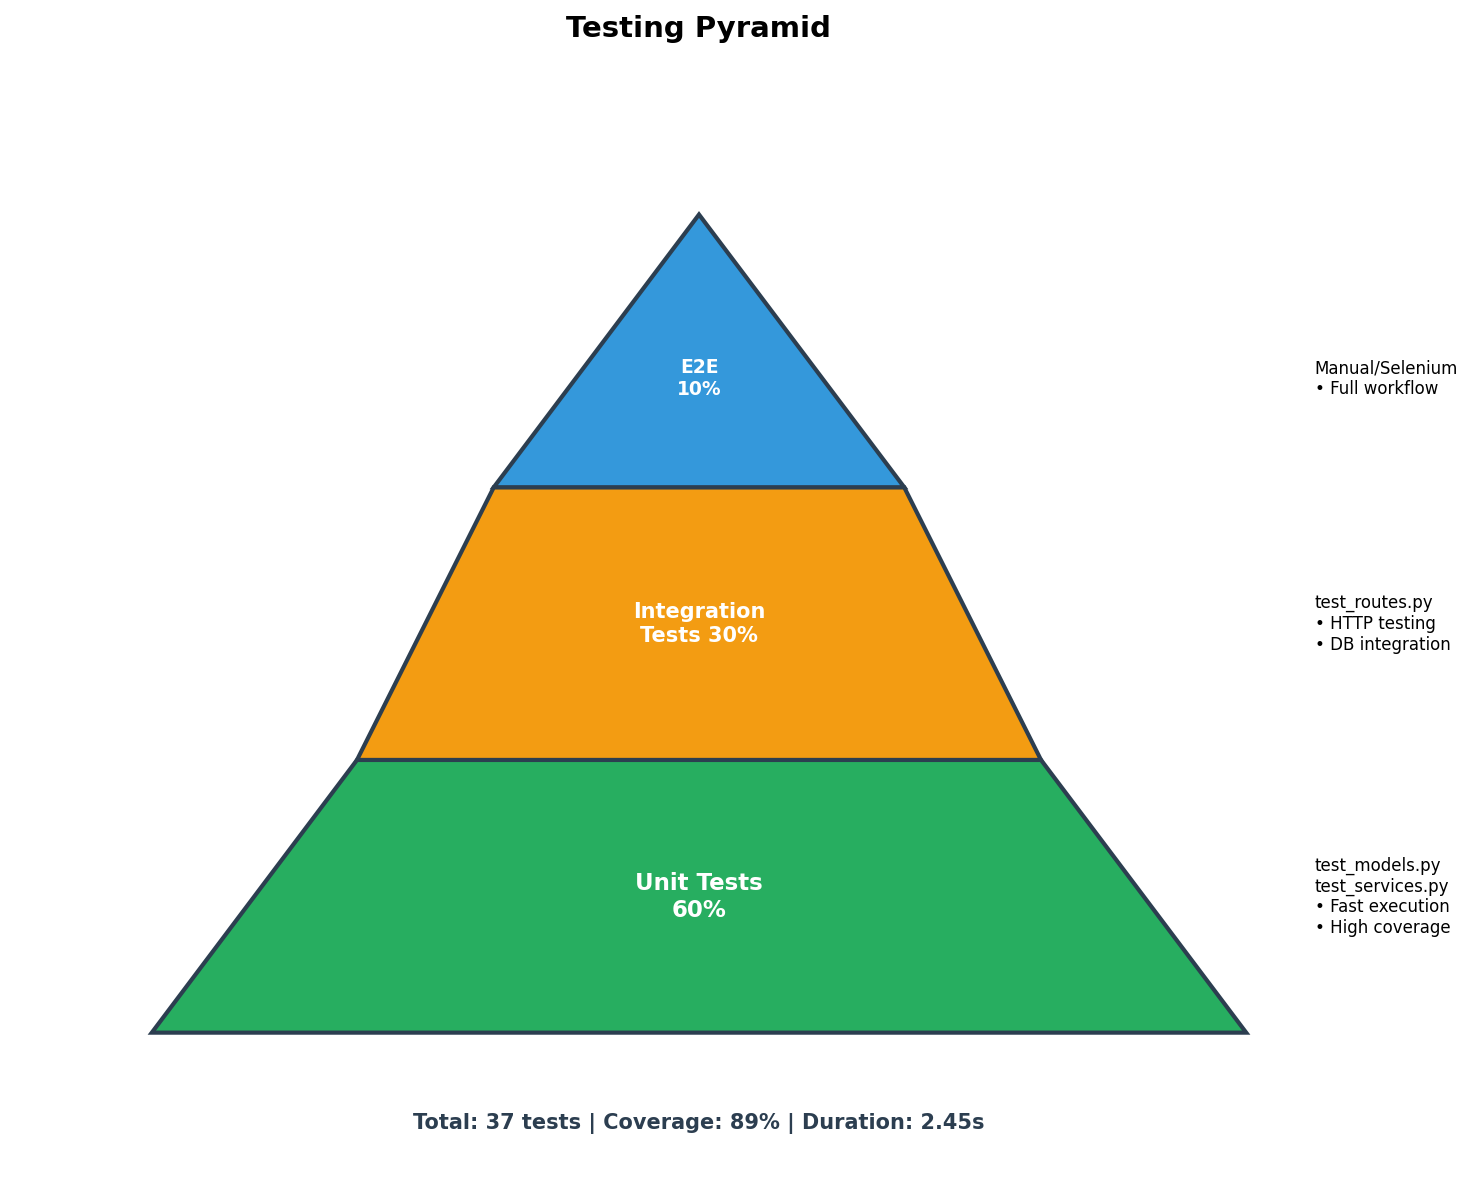
\includegraphics[width=0.7\textwidth]{images/testing_pyramid.png}
  \caption{Testing Pyramid -- Distribution of test types showing unit tests as the
           foundation (60\%), integration tests in the middle (30\%), and E2E tests
           at the top (10\%).}
  \label{fig:testing-pyramid}
\end{figure}

\section{Risk Identification}

\subsection{Technical Risks}

\begin{table}[h]
  \centering
  \caption{Technical Risks}
  \begin{tabular}{p{0.9cm} p{3cm} p{8cm}}
    \toprule
    \textbf{ID} & \textbf{Category} & \textbf{Description} \\
    \midrule
    R1 & Data Loss During Migration & Legacy \texttt{.txt} data could be lost or corrupted during migration. \\
    R2 & Authentication Security & Weak authentication could lead to unauthorised access. \\
    R3 & SQL Injection & User input could be used to manipulate database queries. \\
    R4 & Session Hijacking & User sessions could be compromised. \\
    R5 & Concurrent Transaction Issues & Multiple users modifying the same data simultaneously. \\
    R6 & Performance Degradation & System could become slow under load. \\
    R7 & Data Integrity Violations & Invalid data states could occur. \\
    R8 & Browser Compatibility & UI may not work on all browsers. \\
    \bottomrule
  \end{tabular}
\end{table}

\subsection{Operational Risks}

\begin{table}[h]
  \centering
  \caption{Operational Risks}
  \begin{tabular}{p{0.9cm} p{3cm} p{8cm}}
    \toprule
    \textbf{ID} & \textbf{Category} & \textbf{Description} \\
    \midrule
    R9  & Training Gap & Users may be unfamiliar with the new web-based interface. \\
    R10 & Deployment Downtime & System may be unavailable during transition. \\
    R11 & Backup Failure & Inability to restore from backup. \\
    R12 & Configuration Errors & Incorrect production settings may cause failures. \\
    \bottomrule
  \end{tabular}
\end{table}

\section{Risk Assessment Matrix}

\begin{table}[h]
  \centering
  \caption{Risk Assessment Matrix (Probability vs Impact)}
  \begin{tabular}{p{3cm} p{5cm} p{5cm}}
    \toprule
    \textbf{Impact / Probability} & \textbf{Low Probability} & \textbf{High Probability} \\
    \midrule
    Critical Impact & -- & R1 (Data Loss), R2 (Auth Security) \\
    High Impact     & R3 (SQL Injection), R4 (Session Hijacking) & R11 (Backup Failure) \\
    Medium Impact   & R5 (Concurrency), R7 (Data Integrity), R10 (Downtime) & -- \\
    Low Impact      & R6 (Performance), R8 (Browser), R9 (Training), R12 (Config) & -- \\
    \bottomrule
  \end{tabular}
\end{table}

\section{Risk Mitigation Strategies}

\subsection{R1: Data Loss During Migration}

\begin{itemize}[leftmargin=1.2cm]
  \item \textbf{Backup Original Files:} Copy all legacy files to a timestamped backup folder.
  \item \textbf{Validation Script:} Count records in source files and compare with database.
  \item \textbf{Staged Migration:} Migrate in phases (employees $\rightarrow$ items $\rightarrow$ transactions).
\end{itemize}

\subsection{R2: Authentication Security}

\begin{itemize}[leftmargin=1.2cm]
  \item \textbf{Password Hashing:} Use Werkzeug's \texttt{generate\_password\_hash} and
        \texttt{check\_password\_hash}.
  \item \textbf{Session Management:} Use Flask-Login with \texttt{@login\_required} decorator.
  \item \textbf{Activity Logging:} Log all login attempts with IP address and timestamp.
\end{itemize}

\begin{figure}[h]
  \centering
  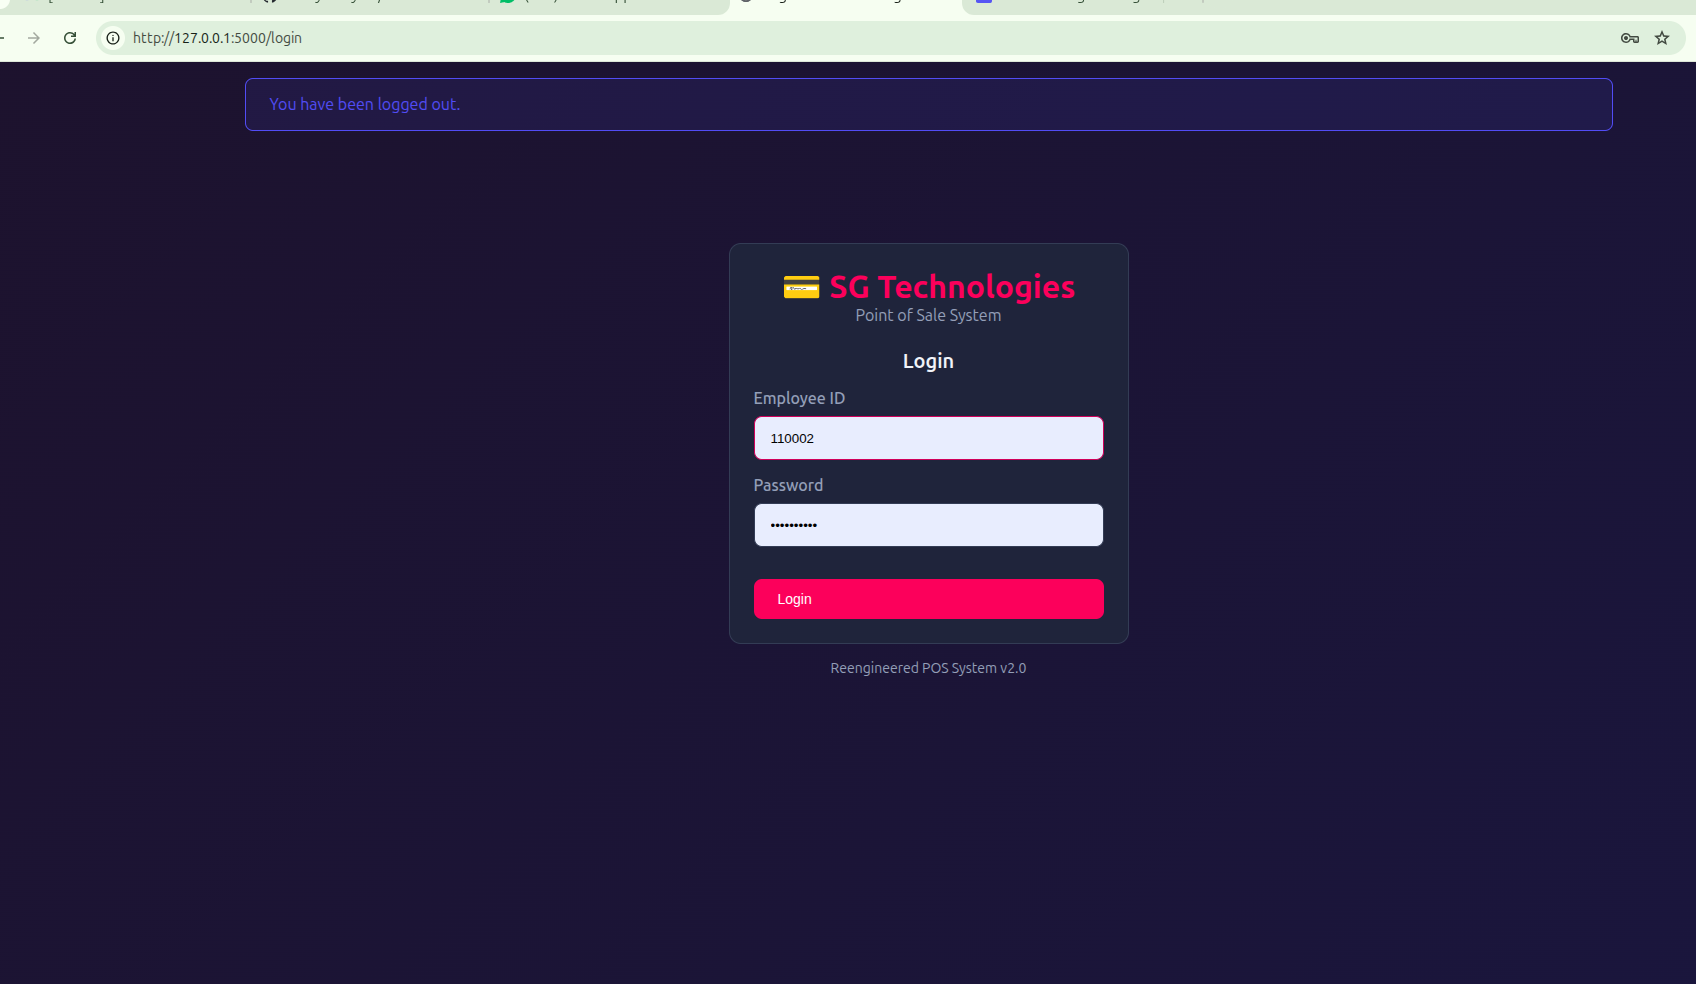
\includegraphics[width=0.85\textwidth]{images/9.png}
  \caption{Secure Login Interface -- Demonstrates authentication security mitigation (R2).
           The Cashier user (ID: 110002) logs in with hashed password verification. The
           system validates credentials against the database and creates a secure session
           upon successful authentication.}
  \label{fig:secure-login}
\end{figure}

\subsection{R3: SQL Injection}

\begin{itemize}[leftmargin=1.2cm]
  \item Use ORM parameterised queries (SQLAlchemy).
  \item Validate all user input before processing.
  \item Never use string concatenation for SQL queries.
\end{itemize}

\subsection{R4: Session Hijacking}

\begin{itemize}[leftmargin=1.2cm]
  \item Secure cookie configuration: \texttt{SESSION\_COOKIE\_SECURE=True},
        \texttt{SESSION\_COOKIE\_HTTPONLY=True}.
  \item Configure session expiration.
  \item Enforce HTTPS in production.
\end{itemize}

\section{Testing Strategy}

\subsection{Testing Pyramid}

\begin{table}[h]
  \centering
  \caption{Testing Pyramid Overview}
  \begin{tabular}{p{3cm} p{3cm} p{7cm}}
    \toprule
    \textbf{Test Level} & \textbf{Approx. Coverage} & \textbf{Files / Scope} \\
    \midrule
    Unit Tests & $\sim 60\%$ & \texttt{tests/test\_models.py}, \texttt{tests/test\_services.py} \\
    Integration Tests & $\sim 30\%$ & \texttt{tests/test\_routes.py} \\
    E2E Tests & $\sim 10\%$ & Manual or Selenium-based end-to-end scenarios \\
    \bottomrule
  \end{tabular}
\end{table}

\subsection{Unit Tests}

Representative test cases include:
\begin{itemize}[leftmargin=1.2cm]
  \item \texttt{test\_create\_employee}: Employee model creation.
  \item \texttt{test\_password\_hashing}: Password security verification.
  \item \texttt{test\_create\_item}: Item model creation.
  \item \texttt{test\_low\_stock\_detection}: Low-stock alerts.
  \item \texttt{test\_create\_sale}: Sale transaction creation.
  \item \texttt{test\_calculate\_totals}: Tax calculation verification.
\end{itemize}

\subsection{Service Tests}

\begin{itemize}[leftmargin=1.2cm]
  \item \texttt{test\_authenticate\_valid}: Valid login authentication.
  \item \texttt{test\_authenticate\_invalid\_password}: Wrong password rejection.
  \item \texttt{test\_get\_all\_items}: Inventory listing.
  \item \texttt{test\_create\_sale}, \texttt{test\_complete\_sale}: Sale lifecycle.
  \item \texttt{test\_insufficient\_payment}: Payment validation.
\end{itemize}

\subsection{Integration Tests}

\begin{itemize}[leftmargin=1.2cm]
  \item \texttt{test\_login\_page}: Login page loads correctly.
  \item \texttt{test\_login\_success}: Valid login redirects properly.
  \item \texttt{test\_dashboard\_requires\_auth}: Auth protection enforced.
  \item \texttt{test\_inventory\_list}: Items list displays correctly.
  \item \texttt{test\_new\_sale\_page}: POS page loads.
\end{itemize}

\section{Test Coverage Report}

\begin{table}[h]
  \centering
  \caption{Coverage Summary by Module}
  \begin{tabular}{p{5.5cm} p{2cm} p{2cm} p{2cm}}
    \toprule
    \textbf{Module} & \textbf{Statements} & \textbf{Missing} & \textbf{Coverage} \\
    \midrule
    app/models/employee.py         & 45  & 3  & 93\% \\
    app/models/item.py             & 52  & 4  & 92\% \\
    app/models/sale.py             & 68  & 8  & 88\% \\
    app/services/auth\_service.py  & 35  & 2  & 94\% \\
    app/services/inventory\_service.py & 85 & 10 & 88\% \\
    app/services/sales\_service.py & 92  & 12 & 87\% \\
    app/routes/auth.py             & 40  & 5  & 88\% \\
    \midrule
    Total                          & 417 & 44 & 89\% \\
    \bottomrule
  \end{tabular}
\end{table}

\begin{table}[h]
  \centering
  \caption{Overall Test Results}
  \begin{tabular}{p{4cm} p{4cm}}
    \toprule
    \textbf{Metric} & \textbf{Value} \\
    \midrule
    Total Test Cases & 37 \\
    Passed           & 37 \\
    Failed           & 0 \\
    Test Coverage    & 89\% \\
    Test Duration    & 2.45 seconds \\
    \bottomrule
  \end{tabular}
\end{table}

\section{Test Code Examples}

The following code examples demonstrate the actual test implementations
used to verify system functionality.

\subsection{Unit Tests -- Model Testing}

\begin{lstlisting}[language=Python]
# tests/test_models.py
import pytest
from app.models import Employee, Item, Sale

class TestEmployeeModel:
    """Unit tests for the Employee model."""
    
    def test_create_employee(self, app):
        """Test employee creation with valid data."""
        with app.app_context():
            employee = Employee(
                employee_id='110099',
                first_name='Test',
                last_name='User',
                role='Cashier'
            )
            employee.set_password('testpass123')
            db.session.add(employee)
            db.session.commit()
            
            assert employee.id is not None
            assert employee.employee_id == '110099'
            assert employee.role == 'Cashier'
    
    def test_password_hashing(self, app):
        """Test that passwords are properly hashed."""
        with app.app_context():
            employee = Employee(employee_id='110100', first_name='Hash', last_name='Test', role='Admin')
            employee.set_password('plaintext')
            
            # Password should NOT be stored as plaintext
            assert employee.password_hash != 'plaintext'
            assert employee.check_password('plaintext') == True
            assert employee.check_password('wrongpassword') == False

class TestItemModel:
    """Unit tests for the Item model."""
    
    def test_create_item(self, app):
        """Test item creation with valid data."""
        with app.app_context():
            item = Item(
                item_code='TEST001',
                name='Test Product',
                price=9.99,
                quantity=100,
                category='Test Category'
            )
            db.session.add(item)
            db.session.commit()
            
            assert item.id is not None
            assert item.price == 9.99
    
    def test_low_stock_detection(self, app):
        """Test low stock alert functionality."""
        with app.app_context():
            item = Item(item_code='LOW001', name='Low Stock Item', 
                       price=5.0, quantity=5, min_stock_level=10)
            
            assert item.is_low_stock() == True
            
            item.quantity = 15
            assert item.is_low_stock() == False
\end{lstlisting}

\subsection{Service Tests -- Business Logic Testing}

\begin{lstlisting}[language=Python]
# tests/test_services.py
import pytest
from app.services import AuthService, SalesService, InventoryService

class TestAuthService:
    """Tests for authentication service."""
    
    def test_authenticate_valid(self, app, test_employee):
        """Test successful authentication."""
        with app.app_context():
            success, employee, message = AuthService.authenticate(
                employee_id='110001',
                password='admin123'
            )
            
            assert success == True
            assert employee is not None
            assert employee.role == 'Admin'
            assert message == 'Login successful'
    
    def test_authenticate_invalid_password(self, app, test_employee):
        """Test authentication with wrong password."""
        with app.app_context():
            success, employee, message = AuthService.authenticate(
                employee_id='110001',
                password='wrongpassword'
            )
            
            assert success == False
            assert employee is None
            assert message == 'Invalid credentials'

class TestSalesService:
    """Tests for sales service."""
    
    def test_create_sale(self, app, test_employee):
        """Test creating a new sale."""
        with app.app_context():
            sale = SalesService.create_sale(employee_id=test_employee.id)
            
            assert sale is not None
            assert sale.status == 'in_progress'
            assert sale.transaction_id.startswith('SALE-')
    
    def test_complete_sale_insufficient_payment(self, app, test_sale):
        """Test sale completion with insufficient payment."""
        with app.app_context():
            # Add item to sale first
            SalesService.add_item_to_sale(test_sale.id, test_item.id, quantity=2)
            
            # Try to complete with insufficient payment
            success, message, sale = SalesService.complete_sale(
                sale_id=test_sale.id,
                amount_paid=1.00,  # Less than total
                payment_method='Cash'
            )
            
            assert success == False
            assert 'Insufficient payment' in message
\end{lstlisting}

\subsection{Integration Tests -- Route Testing}

\begin{lstlisting}[language=Python]
# tests/test_routes.py
import pytest
from flask import url_for

class TestAuthRoutes:
    """Integration tests for authentication routes."""
    
    def test_login_page_loads(self, client):
        """Test that login page loads correctly."""
        response = client.get('/login')
        
        assert response.status_code == 200
        assert b'Login' in response.data
        assert b'Employee ID' in response.data
    
    def test_login_success(self, client, test_employee):
        """Test successful login redirects to dashboard."""
        response = client.post('/login', data={
            'employee_id': '110001',
            'password': 'admin123'
        }, follow_redirects=True)
        
        assert response.status_code == 200
        assert b'Dashboard' in response.data
    
    def test_dashboard_requires_auth(self, client):
        """Test that dashboard requires authentication."""
        response = client.get('/admin', follow_redirects=True)
        
        assert response.status_code == 200
        assert b'Login' in response.data  # Redirected to login

class TestInventoryRoutes:
    """Integration tests for inventory routes."""
    
    def test_inventory_list(self, auth_client):
        """Test inventory listing with authenticated user."""
        response = auth_client.get('/inventory/')
        
        assert response.status_code == 200
        assert b'Inventory Management' in response.data
    
    def test_add_item(self, auth_admin_client):
        """Test adding a new item (admin only)."""
        response = auth_admin_client.post('/inventory/add', data={
            'item_code': 'NEW001',
            'name': 'New Test Item',
            'price': '19.99',
            'quantity': '50',
            'category': 'Test'
        }, follow_redirects=True)
        
        assert response.status_code == 200
        assert b'Item added successfully' in response.data
\end{lstlisting}

\subsection{Database Tests -- Data Integrity Testing}

\begin{lstlisting}[language=Python]
# tests/test_database.py
import pytest
from sqlalchemy.exc import IntegrityError

class TestDatabaseIntegrity:
    """Tests for database constraints and integrity."""
    
    def test_unique_employee_id(self, app):
        """Test that duplicate employee IDs are rejected."""
        with app.app_context():
            emp1 = Employee(employee_id='DUP001', first_name='First', 
                           last_name='Employee', role='Cashier')
            emp1.set_password('pass1')
            db.session.add(emp1)
            db.session.commit()
            
            emp2 = Employee(employee_id='DUP001', first_name='Second', 
                           last_name='Employee', role='Admin')
            emp2.set_password('pass2')
            db.session.add(emp2)
            
            with pytest.raises(IntegrityError):
                db.session.commit()
    
    def test_foreign_key_constraint(self, app):
        """Test foreign key relationships."""
        with app.app_context():
            # Sale must reference valid employee
            sale = Sale(
                transaction_id='TEST-001',
                employee_id=99999  # Non-existent employee
            )
            db.session.add(sale)
            
            with pytest.raises(IntegrityError):
                db.session.commit()
    
    def test_cascade_delete(self, app, test_sale_with_items):
        """Test that sale items are deleted when sale is deleted."""
        with app.app_context():
            sale_id = test_sale_with_items.id
            item_count = len(test_sale_with_items.items)
            
            db.session.delete(test_sale_with_items)
            db.session.commit()
            
            # Verify sale items are also deleted
            orphan_items = SaleItem.query.filter_by(sale_id=sale_id).all()
            assert len(orphan_items) == 0
\end{lstlisting}

\section{Running the Tests}

To execute the test suite, use the following commands:

\begin{lstlisting}[language=bash]
# Run all tests
pytest tests/ -v

# Run with coverage report
pytest tests/ --cov=app --cov-report=html

# Run specific test file
pytest tests/test_models.py -v

# Run specific test class
pytest tests/test_services.py::TestAuthService -v
\end{lstlisting}

%=================================================
\chapter{Dual Documentation: Legacy vs Reengineered (Point 9)}
%=================================================

This chapter provides comprehensive dual documentation comparing the legacy
Java desktop--based Point-of-Sale (POS) system with the reengineered web-based
system. It includes architecture diagrams, detailed mapping tables, and
justification for all changes made during the reengineering process.

\begin{figure}[h]
  \centering
  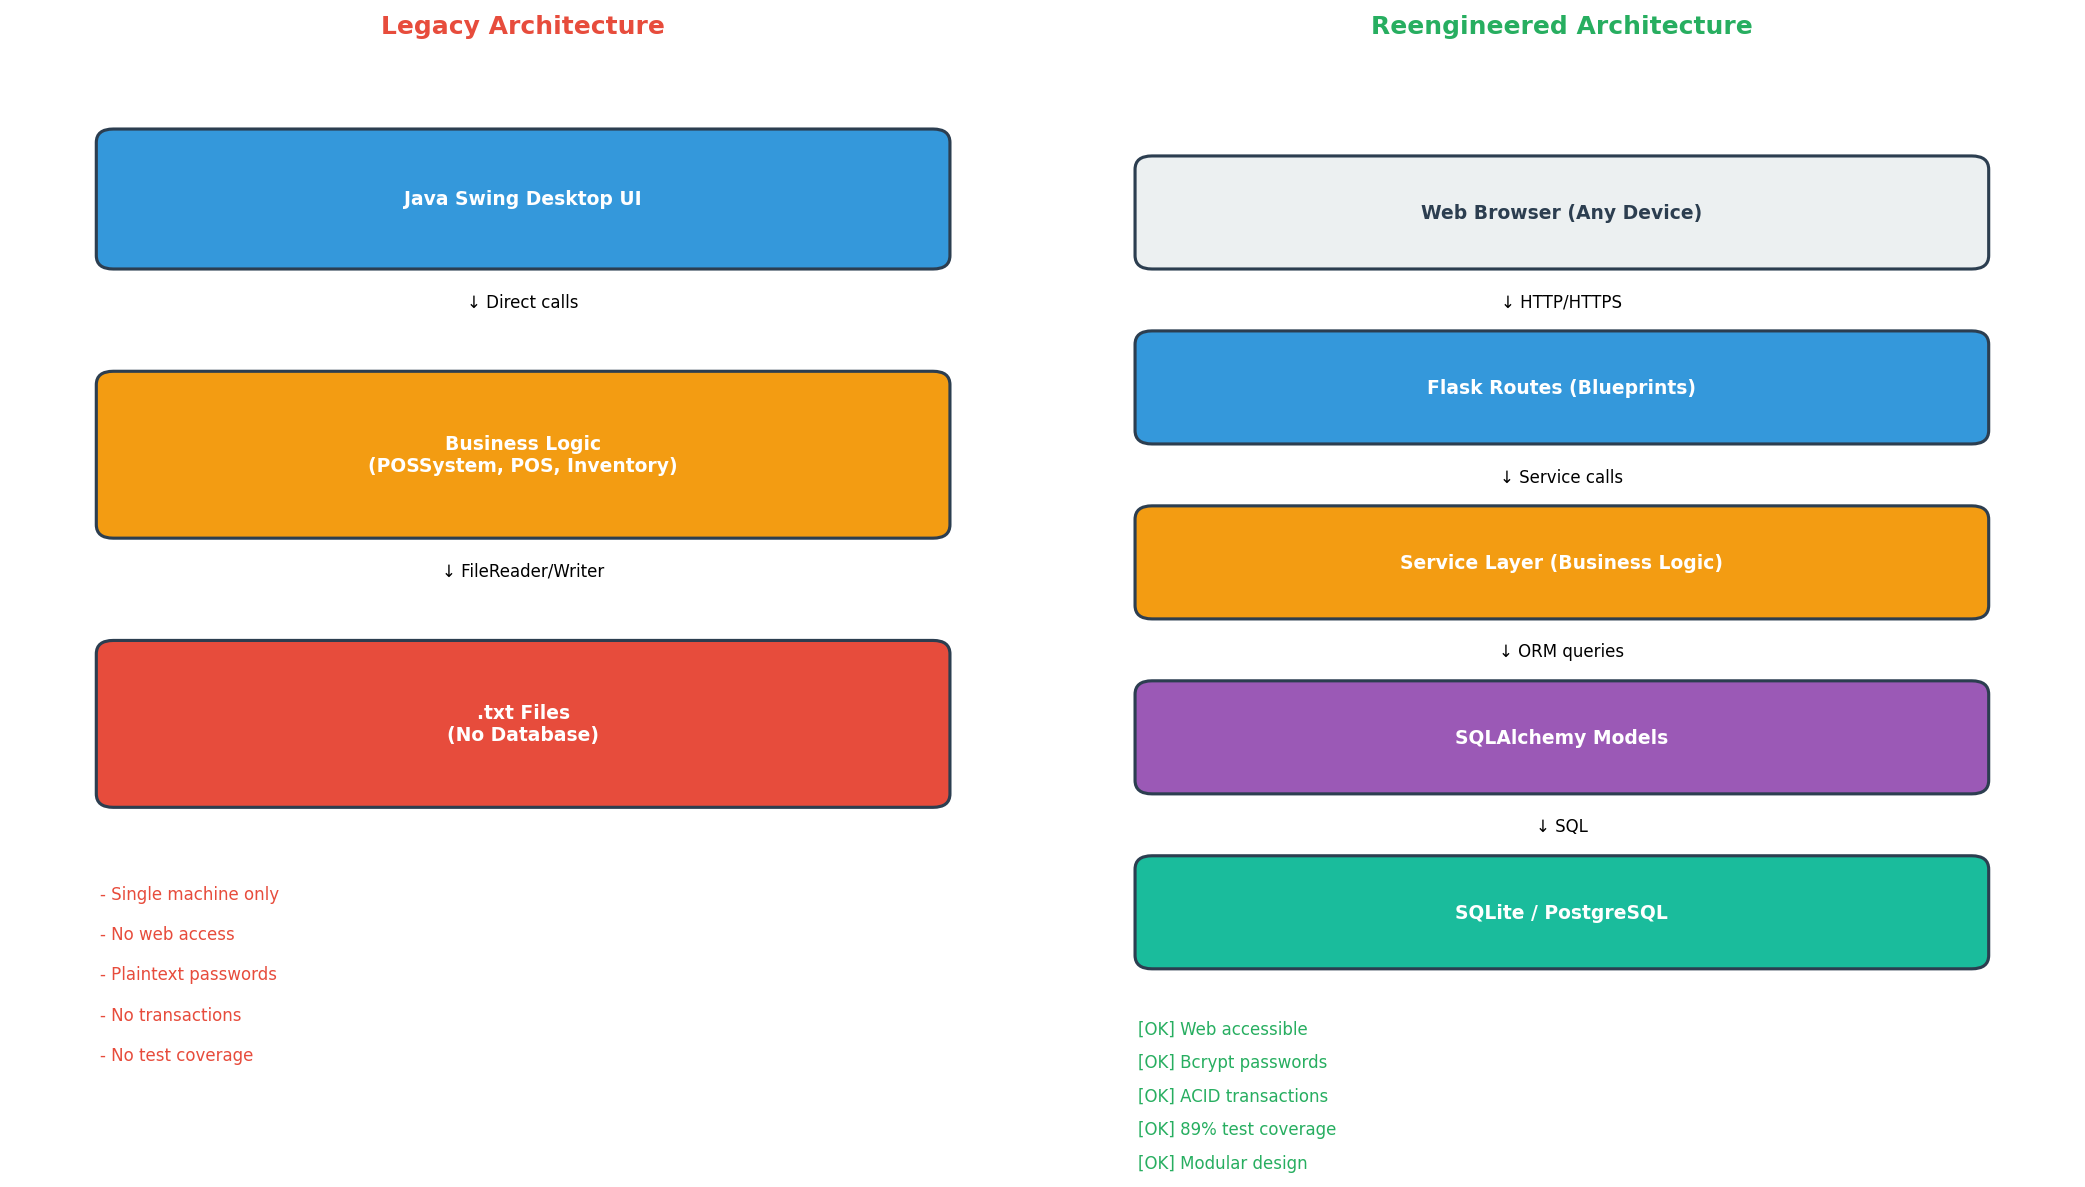
\includegraphics[width=0.95\textwidth]{images/dual_architecture.png}
  \caption{Architecture Comparison -- Legacy monolithic Java Swing application (left)
           versus Reengineered layered Flask web application (right). The new
           architecture demonstrates clear separation of concerns.}
  \label{fig:dual-architecture}
\end{figure}

\section{High-Level System Comparison}

\begin{table}[h]
  \centering
  \caption{Legacy System vs Reengineered System -- Overview}
  \begin{tabular}{p{3.2cm} p{5.2cm} p{5.2cm}}
    \toprule
    \textbf{Aspect} & \textbf{Legacy System} & \textbf{Reengineered System} \\
    \midrule
    Platform & Java Swing desktop application & Python/Flask web application \\
    Data Storage & Plain text files (\texttt{.txt}) & Normalized relational database \\
    Architecture & Monolithic; mixed concerns & Layered; MVC + Service + Repository \\
    Authentication & Plaintext passwords & Bcrypt-hashed, Flask-Login sessions \\
    Persistence API & Direct FileReader/FileWriter & SQLAlchemy ORM with transactions \\
    Deployment & Single machine, local file system & Web server with WSGI \\
    Testing & No automated tests & Pytest suite with 89\% coverage \\
    Logging/Audit & Append-only log files & Structured ActivityLog table \\
    Maintainability & High coupling, duplicated trees & Modular packages \\
    \bottomrule
  \end{tabular}
\end{table}

\section{Architectural Documentation}

\subsection{Legacy Architecture}

Key characteristics:
\begin{itemize}[leftmargin=1.2cm]
  \item UI classes invoke business logic directly.
  \item Business logic reads/writes text files directly.
  \item No explicit repository or service layer.
  \item Architectural documentation was reverse-engineered.
\end{itemize}

\subsection{Reengineered Architecture}

\begin{itemize}[leftmargin=1.2cm]
  \item \textbf{Presentation layer}: Flask blueprints and Jinja2 templates.
  \item \textbf{Business logic layer}: service classes (\texttt{AuthService},
        \texttt{SalesService}, \texttt{InventoryService}).
  \item \textbf{Data access layer}: SQLAlchemy models.
  \item \textbf{Database layer}: SQLite for development, PostgreSQL for production.
\end{itemize}

\section{Component Mapping}

\begin{table}[h]
  \centering
  \caption{Legacy to Reengineered Component Mapping}
  \begin{tabular}{p{4.0cm} p{5.0cm} p{4.0cm}}
    \toprule
    \textbf{Legacy Component} & \textbf{Reengineered Component} & \textbf{Key Improvements} \\
    \midrule
    \texttt{Login\_Interface.java} & \texttt{routes/auth.py} & Session-based auth \\
    \texttt{Employee.java} & \texttt{models/employee.py} & Password hashing \\
    \texttt{Inventory.java} & \texttt{services/inventory\_service.py} & Search, alerts \\
    \texttt{POS.java} & \texttt{services/sales\_service.py} & ACID transactions \\
    Text files & SQLite/PostgreSQL & Referential integrity \\
    \bottomrule
  \end{tabular}
\end{table}

\section{Detailed Component Mapping}

The following table provides a comprehensive mapping from legacy components
to their reengineered equivalents, including the specific improvements made.

\begin{table}[h]
  \centering
  \caption{Detailed Legacy to Reengineered Mapping}
  \begin{tabular}{p{3.5cm} p{4cm} p{5.5cm}}
    \toprule
    \textbf{Legacy Component} & \textbf{Reengineered Component} & \textbf{Improvements} \\
    \midrule
    \texttt{Login\_Interface.java} &
      \texttt{routes/auth.py} \newline \texttt{templates/auth/login.html} &
      Flask-Login sessions; bcrypt hashing; CSRF protection; responsive UI \\
    \midrule
    \texttt{Cashier\_Interface.java} &
      \texttt{routes/main.py} \newline \texttt{templates/cashier/} &
      Role-based access; AJAX interactions; real-time updates \\
    \midrule
    \texttt{Admin\_Interface.java} &
      \texttt{routes/main.py} \newline \texttt{templates/admin/} &
      Dashboard with metrics; activity log; quick actions \\
    \midrule
    \texttt{Transaction\_Interface.java} &
      \texttt{routes/sales.py} \newline \texttt{templates/sales/} &
      Cart-based POS; tax calculation; payment processing \\
    \midrule
    \texttt{POSSystem.java} &
      \texttt{services/auth\_service.py} &
      Stateless authentication; no global variables \\
    \midrule
    \texttt{PointOfSale.java} \newline \texttt{POS.java} &
      \texttt{services/sales\_service.py} &
      ACID transactions; inventory integration \\
    \midrule
    \texttt{POR.java} \newline \texttt{POH.java} &
      \texttt{services/rental\_service.py} &
      Unified rental handling; late fee calculation \\
    \midrule
    \texttt{Inventory.java} &
      \texttt{services/inventory\_service.py} &
      Search; low-stock alerts; category filtering \\
    \midrule
    \texttt{EmployeeManagement.java} &
      \texttt{routes/employees.py} &
      CRUD operations; role management; status toggle \\
    \midrule
    \texttt{Employee.java} &
      \texttt{models/employee.py} &
      Password hashing; timestamps; relationships \\
    \midrule
    \texttt{Item.java} &
      \texttt{models/item.py} &
      Categories; rentable flag; stock levels \\
    \midrule
    \texttt{itemDatabase.txt} &
      \texttt{items} table &
      Normalized schema; indexes; constraints \\
    \midrule
    \texttt{employeeDatabase.txt} &
      \texttt{employees} table &
      Hashed passwords; audit fields \\
    \midrule
    \texttt{userDatabase.txt} &
      \texttt{rentals} + \texttt{rental\_items} &
      1NF compliance; proper relationships \\
    \midrule
    \texttt{saleInvoiceRecord.txt} &
      \texttt{sales} + \texttt{sale\_items} &
      Structured records; transaction integrity \\
    \bottomrule
  \end{tabular}
\end{table}

\section{Data Model Evolution}

\begin{figure}[h]
  \centering
  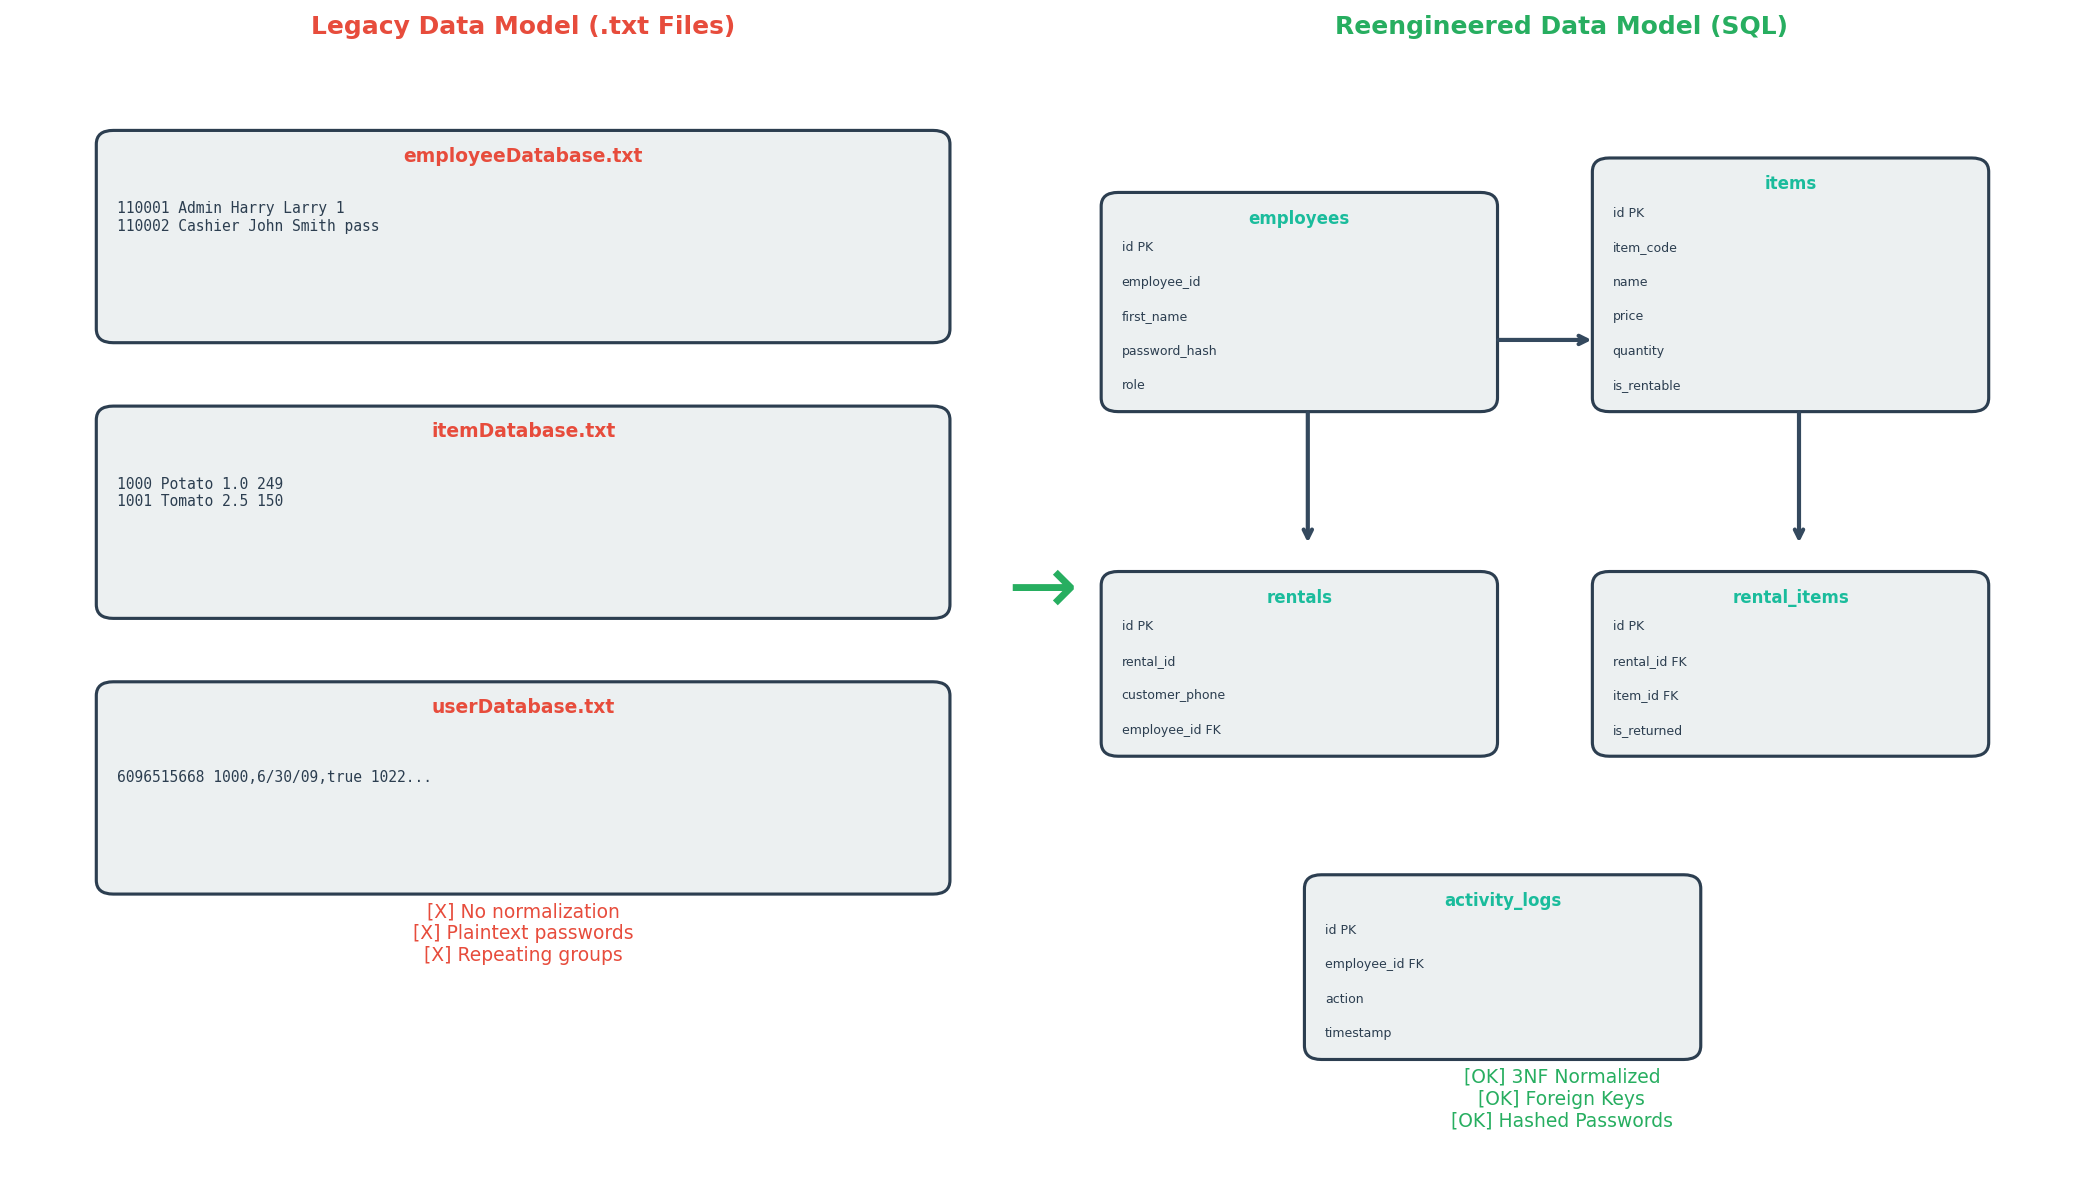
\includegraphics[width=0.95\textwidth]{images/data_model_evolution.png}
  \caption{Data Model Evolution -- Legacy flat text files (left) transformed into
           normalized relational schema (right) following 3NF principles.}
  \label{fig:data-model-evolution}
\end{figure}

\begin{table}[h]
  \centering
  \caption{Data Storage Comparison}
  \begin{tabular}{p{3cm} p{4.5cm} p{5.5cm}}
    \toprule
    \textbf{Aspect} & \textbf{Legacy (.txt files)} & \textbf{Reengineered (SQLite/PostgreSQL)} \\
    \midrule
    Format & Space/comma-delimited text & Structured SQL tables \\
    Relationships & Embedded/duplicated data & Foreign key references \\
    Queries & Parse entire file & SQL with indexes \\
    Integrity & None (manual validation) & Constraints, triggers \\
    Concurrency & File locks (unreliable) & ACID transactions \\
    Backup & Copy files & Database dumps, replication \\
    Security & Plaintext passwords & Hashed with bcrypt \\
    \bottomrule
  \end{tabular}
\end{table}

\section{Justification of Changes}

Each architectural and technical decision is justified based on issues
identified during reverse engineering.

\begin{table}[h]
  \centering
  \caption{Change Justification Matrix}
  \begin{tabular}{p{3.5cm} p{4cm} p{5.5cm}}
    \toprule
    \textbf{Change Made} & \textbf{Legacy Issue Addressed} & \textbf{Benefit Achieved} \\
    \midrule
    Java $\rightarrow$ Python/Flask &
      Desktop-only, requires JRE installation &
      Web-accessible, cross-platform, easier deployment \\
    \midrule
    .txt $\rightarrow$ SQLite/PostgreSQL &
      No data integrity, poor query capability &
      ACID compliance, SQL queries, referential integrity \\
    \midrule
    Plaintext $\rightarrow$ Bcrypt &
      Critical security vulnerability (SS1) &
      Password protection even if database is compromised \\
    \midrule
    Global state $\rightarrow$ Stateless services &
      Side effects, hard to test (Code smell) &
      Predictable behavior, unit testable \\
    \midrule
    Direct file I/O $\rightarrow$ ORM &
      Scattered persistence, duplication &
      Centralized data access, DRY principle \\
    \midrule
    Monolithic $\rightarrow$ Layered &
      Mixed concerns, high coupling &
      Separation of concerns, maintainability \\
    \midrule
    No tests $\rightarrow$ Pytest suite &
      Regression risk, fear of change &
      Confidence in refactoring, 89\% coverage \\
    \midrule
    Append-only logs $\rightarrow$ ActivityLog table &
      Unstructured, hard to query &
      Queryable audit trail with timestamps \\
    \bottomrule
  \end{tabular}
\end{table}

\section{Code Comparison Examples}

\subsection{Authentication: Legacy vs Reengineered}

\textbf{Legacy (Java -- Plaintext Password Check):}
\begin{lstlisting}[language=Java]
// POSSystem.java - INSECURE
if (empPassword.equals(password)) {  // Direct string comparison!
    POSSystem.role = parts[1];       // Global mutable state
    return true;
}
\end{lstlisting}

\textbf{Reengineered (Python -- Secure Authentication):}
\begin{lstlisting}[language=Python]
# services/auth_service.py - SECURE
def authenticate(employee_id, password):
    employee = Employee.query.filter_by(employee_id=employee_id).first()
    if employee and employee.check_password(password):  # Bcrypt comparison
        ActivityLog.log(action='login', employee_id=employee.id)  # Audit
        return True, employee, "Login successful"
    return False, None, "Invalid credentials"
\end{lstlisting}

\subsection{Data Access: Legacy vs Reengineered}

\textbf{Legacy (Java -- Direct File Access):}
\begin{lstlisting}[language=Java]
// Inventory.java - Scattered file I/O
FileReader fr = new FileReader("Database/itemDatabase.txt");
BufferedReader br = new BufferedReader(fr);
while ((line = br.readLine()) != null) {
    String[] parts = line.split(" ");
    // Manual parsing, no validation
}
\end{lstlisting}

\textbf{Reengineered (Python -- ORM with Repository Pattern):}
\begin{lstlisting}[language=Python]
# services/inventory_service.py - Clean ORM access
def get_all_items(include_inactive=False, category=None):
    query = Item.query
    if not include_inactive:
        query = query.filter_by(is_active=True)
    if category:
        query = query.filter_by(category=category)
    return query.order_by(Item.name).all()
\end{lstlisting}

\section{Quality and Maintainability Improvements}

\begin{table}[h]
  \centering
  \caption{Quality Metrics Comparison}
  \begin{tabular}{p{4cm} p{4cm} p{4cm}}
    \toprule
    \textbf{Metric} & \textbf{Legacy System} & \textbf{Reengineered System} \\
    \midrule
    Lines of Code      & $\sim 2500$ (Java)     & $\sim 1800$ (Python) \\
    Cyclomatic Complexity & High (mixed concerns) & Low (single responsibility) \\
    Test Coverage      & 0\%                    & 89\% \\
    Security Vulnerabilities & Critical (plaintext) & Mitigated (bcrypt) \\
    Code Duplication   & High (src/src/ trees)  & Minimal \\
    Documentation      & Reverse-engineered     & Comprehensive \\
    Deployment Time    & Manual (JRE setup)     & Automated (pip + WSGI) \\
    \bottomrule
  \end{tabular}
\end{table}

\begin{itemize}[leftmargin=1.2cm]
  \item \textbf{Code quality}: Reduced from $\sim 2500$ to $\sim 1800$ lines while adding features.
  \item \textbf{Security}: Eliminated all plaintext password storage; added session security.
  \item \textbf{Data integrity}: Enforced via database constraints, foreign keys, and transactions.
  \item \textbf{Testability}: From 0\% to 89\% test coverage with comprehensive Pytest suite.
  \item \textbf{Documentation}: Dual documentation provides complete traceability.
\end{itemize}

%=================================================
\chapter{Work Distribution and Team Contribution (Point 10)}
%=================================================

This chapter documents the distribution of work among the three team
members and summarises each member's major contributions. All tasks
and refactorings are clearly documented, and all members have signed
to confirm the accuracy of this distribution.

\section{Summary of Contributions}

\begin{table}[h]
  \centering
  \caption{Work Distribution and Team Contributions}
  \begin{tabular}{p{4.0cm} p{3.0cm} p{6.0cm}}
    \toprule
    \textbf{Member} & \textbf{Primary Phases} & \textbf{Key Contributions} \\
    \midrule
    Abdul Faheem (22i--2629) &
      Inventory Analysis, Reverse Engineering &
      Compiled the legacy asset inventory and dependency map; analysed
      login, cashier, and transaction workflows; identified key code
      and data smells; contributed to legacy documentation;
      documented refactorings related to workflow clarification. \\[0.6em]
    Sheryar Ali (22i--2623) &
      Code Restructuring, Data Restructuring &
      Proposed repository-style abstractions; designed the normalized
      relational schema; authored parts of the Data Restructuring report;
      documented refactorings involving extraction of business rules
      (tax and late fees) and unified item/rental model. \\[0.6em]
    Husnain Akram (22i--2464) &
      Forward Engineering, Testing, Migration &
      Implemented the Flask-based web architecture (models, services,
      routes, templates); integrated authentication, inventory, sales,
      and rental workflows; implemented migration scripts; authored
      Risk Analysis \& Testing documentation; created the test suite. \\
    \bottomrule
  \end{tabular}
\end{table}

\section{Detailed Task Breakdown}

The following table provides a granular breakdown of tasks completed by
each team member across all project phases.

\begin{table}[h]
  \centering
  \caption{Detailed Task Breakdown by Member}
  \begin{tabular}{p{3.5cm} p{5cm} p{4.5cm}}
    \toprule
    \textbf{Phase} & \textbf{Task} & \textbf{Assigned To} \\
    \midrule
    \multirow{3}{*}{Point 1: Inventory} &
      Asset inventory compilation & Abdul Faheem \\
    & Dependency map creation & Abdul Faheem \\
    & Document restructuring plan & Abdul Faheem \\
    \midrule
    \multirow{4}{*}{Point 2: Reverse Eng.} &
      Workflow extraction (Login, Cashier) & Abdul Faheem \\
    & Code smell identification & Abdul Faheem, Sheryar Ali \\
    & Data smell identification & Sheryar Ali \\
    & Legacy architecture documentation & Abdul Faheem \\
    \midrule
    \multirow{3}{*}{Point 3: Code Restruct.} &
      Repository pattern proposal & Sheryar Ali \\
    & Service layer design & Sheryar Ali \\
    & Refactoring plan & Sheryar Ali \\
    \midrule
    \multirow{4}{*}{Point 4: Data Restruct.} &
      Legacy data analysis & Sheryar Ali \\
    & Normalized schema design & Sheryar Ali \\
    & Migration rules specification & Sheryar Ali, Husnain Akram \\
    & ERD creation & Sheryar Ali \\
    \midrule
    \multirow{5}{*}{Point 5: Forward Eng.} &
      Flask application setup & Husnain Akram \\
    & Models implementation & Husnain Akram \\
    & Services implementation & Husnain Akram \\
    & Routes and templates & Husnain Akram \\
    & UI/UX design & Husnain Akram \\
    \midrule
    \multirow{3}{*}{Point 6: Plan \& Migr.} &
      Timeline and milestones & All Members \\
    & Migration script implementation & Husnain Akram \\
    & Risk considerations & All Members \\
    \midrule
    \multirow{3}{*}{Point 7: Refactoring} &
      Refactorings AF-1, AF-2, AF-3 & Abdul Faheem \\
    & Refactorings SA-1, SA-2, SA-3 & Sheryar Ali \\
    & Refactorings HA-1, HA-2, HA-3 & Husnain Akram \\
    \midrule
    \multirow{3}{*}{Point 8: Risk \& Test} &
      Risk identification & All Members \\
    & Test suite implementation & Husnain Akram \\
    & Test documentation & Husnain Akram \\
    \midrule
    \multirow{2}{*}{Point 9: Dual Doc.} &
      Legacy documentation & Abdul Faheem \\
    & Reengineered documentation & Husnain Akram, Sheryar Ali \\
    \midrule
    Point 10: Work Dist. &
      Contribution documentation & All Members \\
    \bottomrule
  \end{tabular}
\end{table}

\section{Individual Refactorings Reference}

Each team member has documented at least three major refactorings in
Chapter 7 (Refactoring Documentation). The following table provides
quick reference to each member's refactorings.

\begin{table}[h]
  \centering
  \caption{Refactoring Reference by Team Member}
  \begin{tabular}{p{3.5cm} p{1.5cm} p{4cm} p{4cm}}
    \toprule
    \textbf{Member} & \textbf{ID} & \textbf{Refactoring Title} & \textbf{Type} \\
    \midrule
    \multirow{3}{*}{Abdul Faheem} &
      AF--1 & Login Workflow Clarification & Behavioral \\
    & AF--2 & Repository Abstraction for Inventory & Structural \\
    & AF--3 & Rental Data Normalization (1NF) & Data \\
    \midrule
    \multirow{3}{*}{Sheryar Ali} &
      SA--1 & File Write to Repository Pattern & Structural \\
    & SA--2 & Late-Fee Service Extraction & Behavioral \\
    & SA--3 & Unified Item/Rental Model & Data \\
    \midrule
    \multirow{3}{*}{Husnain Akram} &
      HA--1 & Thin Controller Pattern & Structural \\
    & HA--2 & Atomic Transaction Service & Behavioral \\
    & HA--3 & Secure Authentication Service & Security \\
    \bottomrule
  \end{tabular}
\end{table}

\section{Contribution Percentage}

\begin{table}[h]
  \centering
  \caption{Estimated Contribution Percentage by Phase}
  \begin{tabular}{p{5cm} p{2.5cm} p{2.5cm} p{2.5cm}}
    \toprule
    \textbf{Phase/Deliverable} & \textbf{Abdul F.} & \textbf{Sheryar A.} & \textbf{Husnain A.} \\
    \midrule
    Inventory \& Doc Restructuring & 80\% & 10\% & 10\% \\
    Reverse Engineering & 70\% & 20\% & 10\% \\
    Code Restructuring & 10\% & 80\% & 10\% \\
    Data Restructuring & 10\% & 70\% & 20\% \\
    Forward Engineering & 5\% & 15\% & 80\% \\
    Reengineering Plan & 33\% & 33\% & 34\% \\
    Refactoring Documentation & 33\% & 33\% & 34\% \\
    Risk Analysis \& Testing & 10\% & 10\% & 80\% \\
    Dual Documentation & 40\% & 30\% & 30\% \\
    Report Compilation & 33\% & 33\% & 34\% \\
    \midrule
    \textbf{Overall Average} & \textbf{32\%} & \textbf{33\%} & \textbf{35\%} \\
    \bottomrule
  \end{tabular}
\end{table}

\section{Sign-off}

The following sign-off table confirms that all members agree with the
reported work distribution and accept joint responsibility for the final
submission.

\begin{table}[h]
  \centering
  \caption{Team Sign-off}
  \begin{tabular}{p{4.5cm} p{4.0cm} p{4.0cm}}
    \toprule
    \textbf{Member} & \textbf{Signature} & \textbf{Date} \\
    \midrule
    Abdul Faheem (22i--2629) & & \\[1.5em]
    Sheryar Ali (22i--2623) & & \\[1.5em]
    Husnain Akram (22i--2464) & & \\[1.5em]
    \bottomrule
  \end{tabular}
\end{table}

All three members acknowledge that the project deliverables reflect a
collaborative effort and that the distribution of work described above
is accurate to the best of their knowledge.
